\documentclass[12pt, letterpaper]{report}
\usepackage[utf8]{inputenc}
%\usepackage{minted}
%\usemintedstyle{friendly}
\usepackage{listings}
\usepackage{xcolor}
\usepackage{blindtext}
\usepackage{numprint}
\npthousandsep{\,}
\usepackage{hyperref}
\usepackage{graphicx}
\graphicspath{ {./img/} }
\usepackage{float}
\usepackage[autostyle]{csquotes}  

% Listing

\definecolor{codegreen}{rgb}{0,0.6,0}
\definecolor{codegray}{rgb}{0.5,0.5,0.5}
\definecolor{codepurple}{rgb}{0.58,0,0.82}
\definecolor{backcolour}{rgb}{0.95,0.95,0.92}

% Gruvbox colors
\definecolor{dark0_hard}{RGB}{29,32,33}
\definecolor{dark0}{RGB}{40,40,40}
\definecolor{dark0_soft}{RGB}{50,48,47}
\definecolor{dark1}{RGB}{60,56,54}
\definecolor{dark2}{RGB}{80,73,69}
\definecolor{dark3}{RGB}{102,92,84}
\definecolor{dark4}{RGB}{124,111,100}
\definecolor{gray_245}{RGB}{146,131,116}
\definecolor{gray_244}{RGB}{146,131,116}
\definecolor{light0_hard}{RGB}{249,245,215}
\definecolor{light0}{RGB}{251,241,199}
\definecolor{light0_soft}{RGB}{242,229,188}
\definecolor{light1}{RGB}{235,219,178}
\definecolor{light2}{RGB}{213,196,161}
\definecolor{light3}{RGB}{189,174,147}
\definecolor{light4}{RGB}{168,153,132}
\definecolor{bright_red}{RGB}{251,73,52}
\definecolor{bright_green}{RGB}{184,187,38}
\definecolor{bright_yellow}{RGB}{250,189,47}
\definecolor{bright_blue}{RGB}{131,165,152}
\definecolor{bright_purple}{RGB}{211,134,155}
\definecolor{bright_aqua}{RGB}{142,192,124}
\definecolor{bright_orange}{RGB}{254,128,25}
\definecolor{neutral_red}{RGB}{204,36,29}
\definecolor{neutral_green}{RGB}{152,151,26}
\definecolor{neutral_yellow}{RGB}{215,153,33}
\definecolor{neutral_blue}{RGB}{69,133,136}
\definecolor{neutral_purple}{RGB}{177,98,134}
\definecolor{neutral_aqua}{RGB}{104,157,106}
\definecolor{neutral_orange}{RGB}{214,93,14}
\definecolor{faded_red}{RGB}{157,0,6}
\definecolor{faded_green}{RGB}{121,116,14}
\definecolor{faded_yellow}{RGB}{181,118,20}
\definecolor{faded_blue}{RGB}{7,102,120}
\definecolor{faded_purple}{RGB}{143,63,113}
\definecolor{faded_aqua}{RGB}{66,123,88}
\definecolor{faded_orange}{RGB}{175,58,3}

% Gruvbox Light
\lstdefinestyle{gruvbox_light}{
    backgroundcolor=\color{light0},
    basicstyle=\color{dark0}\ttfamily\footnotesize,
    commentstyle=\color{gray_245},
    keywordstyle=\color{faded_red},
    numberstyle=\tiny\color{faded_orange},
    stringstyle=\color{faded_green},
    breakatwhitespace=false,
    breaklines=true,
    captionpos=b,
    keepspaces=true,
    numbers=left,
    numbersep=5pt,
    showspaces=false,
    showstringspaces=false,
    showtabs=false,
    tabsize=4
}

% Gruvbox Dark
\lstdefinestyle{gruvbox_dark}{
    backgroundcolor=\color{dark0},
    basicstyle=\color{light0}\ttfamily\footnotesize,
    commentstyle=\color{grey_244},
    keywordstyle=\color{bright_red},
    numberstyle=\tiny\color{bright_orange},
    stringstyle=\color{bright_green},
    breakatwhitespace=false,
    breaklines=true,
    captionpos=b,
    keepspaces=true,
    numbers=left,
    numbersep=5pt,
    showspaces=false,
    showstringspaces=false,
    showtabs=false,
    tabsize=4
}

\lstdefinestyle{mystyle}{
    backgroundcolor=\color{backcolour},   
    commentstyle=\color{codegreen},
    keywordstyle=\color{magenta},
    numberstyle=\tiny\color{codegray},
    stringstyle=\color{codepurple},
    basicstyle=\ttfamily\footnotesize,
    breakatwhitespace=false,         
    breaklines=true,                 
    captionpos=b,                    
    keepspaces=true,                 
    numbers=left,                    
    numbersep=5pt,                  
    showspaces=false,                
    showstringspaces=false,
    showtabs=false,                  
    tabsize=4
}

\lstset{style=gruvbox_light}

% Meta
\title{SQL Training}
\author{Kevin Gilson}
\date{\today{}}

% Document
\begin{document}

% Cover page
\maketitle

% Abstract
\begin{abstract}
This document has for purpose to give its reader a basic introduction to \textbf{DataBases} and \textbf{SQL}, with a focus on \textit{Oracle} databases and syntax.
It will go over the process of querying, selecting, filtering, and grouping data, alongside how to practice theses concept in a safe playground environment.
It is not directed to DBA or more advanced users, and won't cover topics outside of querying data and creating simple tables.
\end{abstract}

% Table of Contents
\tableofcontents

% Theory
\part{Theory}

\chapter{Introduction}

In a world more and more digitalized, \textit{data} has quickly become a hot topic.
From its collection to its utilization, going over its retention, it is now essential to understand how to interact with it.

\section{What are databases}

If we want to truly understand what is behind our day-to-day utilization of data, the first question to ask ourselves is: \textit{What is a database?}

A \textbf{database} is an \textit{organized collection} of structured information, of \textit{data}.

It is often controlled by a \textit{DataBase Management System} (DBMS), and is typically modelled in rows and columns.

\subsection{Differences with MS Excel}

You might ask yourselves \textit{If a database store information in rows and columns, how is it different from Excel?}

From a modelling point of view, it is not.

But from an implementation one, everything change.

Spreadsheets are designed to store a limited amount of data, accessed by one user at the time. Hence, they are also limited in they storage, and can't hold more than \numprint{1048576} rows.

Databases are designed to hold much larger contents; they are not restricted to a finite number of rows.
Moreover, they allow multiple users to quickly, and securely, access and query data using highly complex logic.

As an additional point, they provide an enhance security, and they often require dedicated access for the users, allow for querying logs, and anonymization of sensitive data.

\subsection{Main actors}

Due to its commercial use, databases are highly developed between different providers, the main ones being:
\begin{itemize}
	\item Microsoft SQL Server;
	\item Oracle;
	\item SQL Lite;
	\item MySQL;
	\item MongoDB;
	\item PostgreSQL;
	\item SAP Sybase.
\end{itemize}

In this document, we will focus on \textit{Oracle} databases and syntax, as it is the most widely available and used in the Financial Industry.

\subsection{NO SQL}

Most database are best described has \textit{relational database}, meaning that they follow the classic model of matrices, with rows and columns.

There is another type of databases called \textit{NoSQL}, and act as a storage interface, allowing to store, depending on the solution, whole documents, images, audio-video files, and... \textit{whole databases}.

In this document, we will focus on relational databases.

\section{What is SQL}

Databases represent the \textit{storage} of data. But how do we \textit{access} them?
That is where SQL comes into place.

SQL stands for \textit{Structured Query Language} and is the standard way of communicating with a database.

It can retrieve data from a database, create and update it.

SQL is a default standard more than a language, as each and every provider adapt it to its own model, which can lead to differences in functions (e.g. the \textit{NVL} function exist in Oracle and not in MySQL).

Nevertheless, most of the structure remains the same.

Once again, this document will emphasise the use of \textit{Oracle} SQL.

\chapter{Prerequisites}

Like every programming languages, SQL can not be learning properly without practice.
Luckily for us, it is a widely known and used language, and tools are available for free online.

\section{Oracle LiveSQL}

% Figures don't display correctly
Oracle provide an online querying tool, \textit{LiveSQL}, that can be found \href{https://livesql.oracle.com}{here}.
To follow this guide, please register for the access by clicking on the \textit{Sign In} button:

\begin{figure}[H]
	\centering
	
\includegraphics[width=0.5\textwidth]{livesql_signin}
	\caption{Sign-in}
\end{figure}

Then \textit{Create Account}:

\begin{figure}[H]
	\centering
	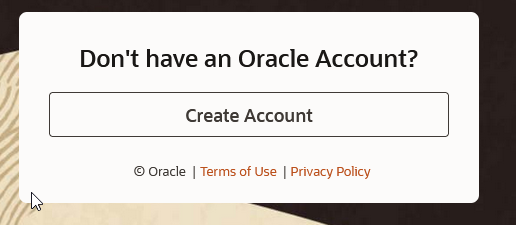
\includegraphics[width=0.5\textwidth]{livesql_create_account_01}
	\caption{Create account}
\end{figure}

Complete the form, then click \textit{Create Account} a second times:

\begin{figure}[H]
	\centering
	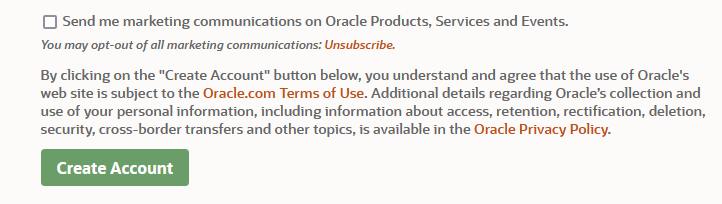
\includegraphics[width=0.5\textwidth]{livesql_create_account_02}
	\caption{Create account}
\end{figure}

And that's it, you are now registered.
Once you connect, click on \textit{Start Coding} to proceed further:

\begin{figure}[H]
	\centering
	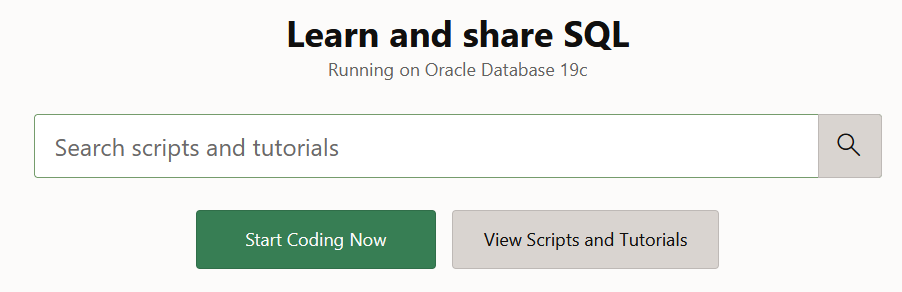
\includegraphics[width=0.5\textwidth]{livesql_start_coding}
	\caption{Accessing the code environment}
\end{figure}

You will then be redirected to the database query editor.
The top frame is where you can input your code:

\begin{figure}[H]
	\centering
	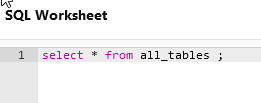
\includegraphics[width=0.5\textwidth]{livesql_code}
	\caption{Accessing the code environment}
\end{figure}

The bottom frame display your result:

\begin{figure}[H]
	\centering
	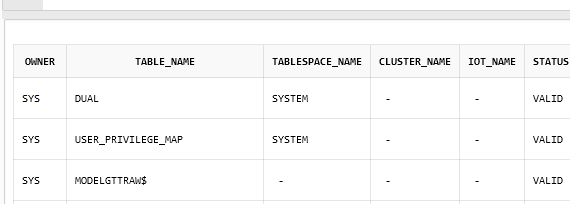
\includegraphics[width=0.5\textwidth]{livesql_output}
	\caption{Accessing the code environment}
\end{figure}

And on the top right, you can see various actions, the most useful one being the number of displayed results:

\begin{figure}[H]
	\centering
	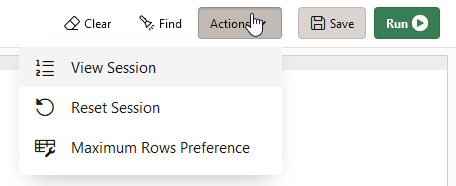
\includegraphics[width=0.5\textwidth]{livesql_actions}
	\caption{Accessing the code environment}
\end{figure}

In order to run a query, simply click \textit{Run}, or press CTRL-Enter.

\section{Oracle Sample Databases}

In order to facilitate the training of new resources, Oracle provide \href{https://docs.oracle.com/database/121/COMSC/overview.htm#COMSC005}{Sample Databases}.
Theses databases are available for free to any company using Oracle as its service provider, and are also the one accessible through \textit{LiveSQL}.

Here is a short description provided by \href{https://docs.oracle.com/database/121/COMSC/overview.htm#COMSC005}{Oracle itself}:
\blockquote{
The sample database schemas provide a common platform for examples in each release of the Oracle Database. The sample schemas are a set of interlinked database schemas. This set provides approach to complexity:
\begin{itemize}
	\item Schema Human Resources (HR) is useful for introducing basic topics. An extension to this schema supports Oracle Internet Directory demos.
	\item Schema Order Entry (OE) is useful for dealing with matters of intermediate complexity. Many data types are available in this schema, including nonscalar data types.
	\item Schema Online Catalog (OC) is a collection of object-relational database objects built inside schema OE.
	\item Schema Product Media (PM) is dedicated to multimedia data types.
	\item A set of schemas gathered under the main schema name Information Exchange (IX) can be used to demonstrate Oracle Advanced Queuing capabilities.
	\item Schema Sales History (SH) is designed to allow for demos with large amounts of data. An extension to this schema provides support for advanced analytic processing.
\end{itemize}
}

For our example, we will use these sample tables.

\chapter{Selecting data}
\section{Anatomy}

A basic SQL query typically looks like this:
\lstinputlisting[language=SQL, caption=Anatomy of a query]{sql/anatomy.sql}

Now let's analyse it a bit.
\begin{itemize}
	\item The query starts with the \textbf{select} keyword; it is the indication given to the database that we want to \textit{view} data, and not \textit{modify} it.
	\item When a user want to avoid potential duplicates, he will perform a  \textbf{select distinct}.
	\item Afterwards, the columns to be displayed are specified the ones after the others; each columns should be separated by a \textbf{comma}.
	Whenever an user want to display the complete set of columns, the list of columns can be replace with a \textit{wildcard}, \textbf{*}.
	\item In this example, we can see that one column is \textit{aggregated} with a \textbf{sum}; this one is enclave between the parentheses of the function.
	The resulting column is \textit{renamed} by using an \textit{alias}, with the \textbf{as} keyword.
	\item Once the columns have been defined, the \textbf{from} keyword starts the selection of the \textit{database}.
	\item The database identifier is always composed of a \textbf{schema}, and a \textbf{table name}, separated by a period.
	\item The \textbf{where} clause is used to filter data, either \textit{string} columns, within \textit{single quotation marks}, or \textit{numbers}.
	Conditions are separated by mathematical operators such as \textbf{and} and \textbf{or}.
	\item When one or more columns are aggregated, a \textbf{group by} clause is mandatory.
	This clause must contain all \textit{non-aggregated} columns that are selected.
	\item To conclude, an \textbf{order by} clause let the user order the results on a column-based, either by \textit{ascending} order (the default value), or \textit{descending}.
	\item It is important to note that a query finish by a \textbf{semi-colon}, which is the indicator for the executor to stop reading.
\end{itemize}

In addition, \textbf{comments} can be add to a SQL query:
\begin{itemize}
	\item Lines starting with \textbf{double dash} \textit{--} will be commented.
	\item A \textbf{Slash followed by a wildcard} \textit{/*} will start a block comment;
	another \textbf{wildcard followed by a slash} \textit{*/} will end it.
\end{itemize}

\section{Formatting}

SQL is case-insensitive, meaning that keywords, column names, schemas, table names, and pretty much everything \textbf{except} conditions values, can be written in \textit{UPPERCASE} or \textit{lowercase}.

It is important to find its own preference and stick to it. I personally write everything in lower case, except for columns that I put in upper case:
\lstinputlisting[language=SQL, caption=My personal preference]{sql/formating.sql}

Each sub-section of the query is indented, making the separations easier on see.

You will also notice that I put each column on a new line, and start this line with the separator, whether in the \textit{select}, \textit{where}, or other clauses.
The purpose of doing this is to be able to easily comment lines when writing and debugging a query.

Often, your first column will be one that you won't touch (a \textit{date} for example), but you might want to periodically add or remove the other ones.
Putting the separator at the beginning of the line allows for commenting that line without breaking your code, while if you had put it at the very end, commenting the last line would raise an error.

\section{Good practices}

Due to the case-insensitive nature of SQL, one could be tempted to mix between cases, but I would advised against it.

The bigger your queries will become, the easier it will be for you to analyse, modify, and debug them, if you remain consistent.

\begin{itemize}
	\item Keep the same formatting alongside your whole query.
	\item Indent your code; it make it more readable.
	\item Use comments; a good comment should be long enough to describe, but short enough that it doesn't cluster your screen.
	\item Favor 3-4grams aliases, it lines up better, it is easier to remember, and it takes less screen space.
	
	Example: a table \textit{Customer} would become \textit{cus}, \textit{Order} would become \textit{ord}, etc.
	\item Always alias your tables. While it might seems useless when you are only querying a single table, it will comes up in handy when you decide to adapt that query and add joins.
	\item Use \textbf{bind variables}. In SQL, a bind variable is a keyword defined by \textbf{a colon followed by this keyword}, such as \textit{:querying\_period}.
	You can use bind variables within your \textit{where} clause, and each time you will run your query, Oracle will require you to input the corresponding value for that parameter.
	In term of execution time, bind variable might increase the performances of your queries.

	\textit{This functionality might not be accessible in Oracle LiveSQL.}
	
	\item Avoid \textit{select *} as much as your can. Use it to explore a table quickly, then develop your query with given columns.
	\item Maths also apply in SQL: when you use multiple conditions within your \textit{where} clause, the order of operation apply. Use parentheses to capitalise on it.
	\item Most databases tables contains  \textit{at least} one \textbf{primary key}, which is an unique ID. This ID is \textit{indexed}, meaning that the database knows precisely the position of each records based on that ID.
	
	A specific table can contain several indexes; it is important to get to know the indexes of your tables, and filter on them. This should greatly improve your queries performances.
\end{itemize}

\section{Oracle internal tables - Your first select}

As described above, the process of a simple select is quite straightforward: \textit{select * from schema.table}.

But when dealing with a new environment, it might be though to now \textit{on which} table to look at. That is where Oracle internal tables comes in handy.

Each Oracle database contains several internal tables, out of which five are particularly interesting:
\begin{itemize}
	\item \textbf{all\_tables} contains a list of all \textit{schema}, and their relative \textit{tables}, within the connection you are running it on.
	\item \textbf{all\_views} is identical, except that it focus on \textit{views}.
	
	\textit{For most basic users, the difference between tables and views is not worth mentioning. Just realise that if you don't find any tables in the first one, you are likely to only have access to views and should use the second one.}
	
	\item \textbf{all\_tab\_columns} contains both tables and views, alongside all their respective \textit{columns}.
	\item \textbf{all\_tab\_comments} contains both tables and views, alongside a \textit{comment} on what they represent.
	\item \textbf{all\_col\_comments} is identical, except that the \textit{comment} refer to each columns of the given table.
\end{itemize}

\textit{Comments are defined by the DBA. Depending on the environment you are running your queries on, it might be empty.}

By performing queries on theses various tables, you are likely to understand better your current connection, and can also look for specific tables, columns, etc, based on quick SQL queries.

To get familiar with them, run the following query on LiveSQL and explore the available tables:
\lstinputlisting[language=SQL, caption=LiveSQL Tables]{sql/all_tables.sql}

This query filter on tables that are \textbf{not} part of the internal Oracle system.

As a bonus, the following query will most likely return you all the available tables in a simpler manner:
\lstinputlisting[language=SQL, caption=LiveSQL Tables - Simple]{sql/all_tables_bonus.sql}

Feel free to explore the LiveSQL datasets that you will find in the results.

\chapter{Filtering with the Where clause}

Once you have selected your columns, and table, you will probably want to filter on specific results; that is when the \textbf{where} clause comes in handy.

In SQL, the \textit{where} clause mark the beginning of query conditions.

\section{Equalities}

\textbf{Equalities} are pretty simple: you either use an \textit{equal sign} \textbf{=} to display an equality, or \textit{two chevrons} \textbf{<>} to display a difference.

\textit{(N.B.: A difference can also be displayed by an exclamation mark followed by an equal sign, !=; I would advise to pick one of the method and stick with it. Alongside this document, I will keep using the dual chevrons.}

A part from that, only one point should be taken into account: whether the equality refers to a string, or a number.

\begin{itemize}
	\item When referring to a \textit{string}, the value should be enclosed between single quotation marks.
	\item When referring to a \textit{number}, the value can be input directly.
\end{itemize}

There is also a third option: comparing one column with another. In this case, no quotation marks should be used, and both columns should be called the same way you would call them in any other clause.

Here is a few example of equalities:

\lstinputlisting[language=SQL, caption=String equality]{sql/string_equality.sql}

\lstinputlisting[language=SQL, caption=String difference]{sql/string_difference.sql}

\lstinputlisting[language=SQL, caption=Number equality]{sql/number_equality.sql}

\lstinputlisting[language=SQL, caption=Number difference]{sql/number_difference.sql}

\lstinputlisting[language=SQL, caption=Columns equality]{sql/columns_equality.sql}

\lstinputlisting[language=SQL, caption=Columns difference]{sql/columns_difference.sql}

\section{Inequalities}

\textbf{Inequalities} follows the exact same principle as equalities.
Various mathematical inequalities can be used in SQL:

\begin{itemize}
	\item Strictly greater / smaller, depending on the chevron used: \textit{a \> b}
	\item Greater / smaller or equal: \textit{a \>= b}
\end{itemize}

Here is two example displaying theses possibilities:

\lstinputlisting[language=SQL, caption=Strictly Greater than]{sql/greater_than.sql}

\lstinputlisting[language=SQL, caption=Lower or equal than]{sql/lower_or_equal.sql}

\section{Ranges}

Ranges can be defined in two ways in SQL:

\begin{itemize}
	\item Using two \textit{inequalities} with each other.
	\item Using the \textit{between} keyword.
\end{itemize}

As example, the same filter can be expressed with inequalities:
\lstinputlisting[language=SQL, caption=Range - Inequalities]{sql/range_inequalities.sql}

Or with a \textit{between}:
\lstinputlisting[language=SQL, caption=Range - Between]{sql/range_between.sql}

\section{Membership}

In SQL, a membership is defined as whether or not a column value is part of a list.
This list is defined between parentheses after the \textbf{in} keyword.

Within the parentheses, the same rules applies: strings within quotation marks, and number not.
The separator between the different values possible remains the same, a \textit{comma}.

\lstinputlisting[language=SQL, caption=Membership]{sql/membership.sql}

As for the rest of the query, I would advise you to put each possibility on a new line; it will be easier to comment it out.
If your list appears too long to proceed this way, it is often an indicator that you \textit{shouldn't} be filtering this way, and that you should think about reworking your query.

In opposition, we can also filter on \textit{non-membership}, using the \textbf{not} keyword.
The \textit{not} keyword in SQL is used to negate the following condition. Used before an \textit{in}, it will tell SQL to look for column values that are \textit{not} within that list:

\lstinputlisting[language=SQL, caption=Membership]{sql/non_membership.sql}

\section{Pattern matching}
\blindtext

\section{Multiple conditions}
\blindtext

\chapter{Grouping and Ordering}
\section{Group by clause}
\blindtext

\subsection{Sum}
\subsection{Count}
\subsection{Avg}
\subsection{Min}
\subsection{Max}

\section{Having clause}
\blindtext

\section{Order by clause}
\blindtext

\chapter{Joins}
\blindtext

\section{Inner join}
\blindtext

\section{Left and Right Outer join}
\blindtext

\section{Full Outer join}
\blindtext

\section{Oracle specific syntax}
\blindtext

\chapter{Handling null values}
\blindtext

\section{Is Null}
\blindtext

\section{NVL}
\blindtext

\section{NVL2}
\blindtext

\section{COALESCE}
\blindtext

\chapter{Case-When}
\blindtext

\section{Basic syntax}
\blindtext

\section{Multiple conditions syntax}
\blindtext

\section{Aggregated results syntax}
\blindtext

\chapter{Format Operations}
\blindtext

\section{Numerical Operations}
\blindtext

\subsection{Round}
\subsection{Greatest and Least}

\section{String Operations}
\blindtext

\subsection{To\_String}
\subsection{Concatenation}
\subsection{LPAD and RPAD}

\section{Date Operations}
\blindtext

\subsection{To\_Date}
\subsection{Add\_Months}

\chapter{Partition by}
\blindtext

\section{ROW\_NUMBER}
\blindtext

\section{LIST\_AGG}
\blindtext

\chapter{Sub-queries}
\blindtext

\section{The classical approach}

\section{The With clause}

% Already covered in the Good practices
%\chapter{Bind variables}

%\chapter{Pivot}

%\chapter{Create, Drop, and Alter Table}

% Exercises
\part{Exercises}
\section{Schema CO}
\subsection{}
\lstinputlisting[language=SQL, caption=Anatomy of a query]{sql/anatomy.sql}

\section{Schema HR}
\section{Schema OE}

% Solution
\part{Solutions}
\section{Schema CO}
\section{Schema HR}
\section{Schema OE}

\end{document}
